\documentclass[conference]{IEEEtran}
\IEEEoverridecommandlockouts
% The preceding line is only needed to identify funding in the first footnote. If that is unneeded, please comment it out.
\usepackage{cite}
\usepackage{amsmath,amssymb,amsfonts}
\usepackage{algorithmic}
\usepackage{textcomp}

% Muz packages
\usepackage{graphicx}
\usepackage{lineno}
\usepackage{color}
% \usepackage{amsmath} added above
\usepackage{comment}
\usepackage{setspace}

% \doublespacing

\def\BibTeX{{\rm B\kern-.05em{\sc i\kern-.025em b}\kern-.08em
    T\kern-.1667em\lower.7ex\hbox{E}\kern-.125emX}}
\begin{document}

\title{A deep learning approach to trespassing detection using video surveillance data}

\author{
\IEEEauthorblockN{Muzammil Bashir}
\IEEEauthorblockA{
\textit{Department of Computer Science} \\
\textit{Worcester Polytechnic Institute}\\
United States \\
mbashir@wpi.edu}
\and
\IEEEauthorblockN{Elke A. Rundensteiner}
\IEEEauthorblockA{
\textit{Department of Computer Science} \\
\textit{Worcester Polytechnic Institute}\\
United States \\
rundenst@wpi.edu}
\and
\IEEEauthorblockN{Ramoza Ahsan}
\IEEEauthorblockA{
\textit{Department of Computer Science} \\
\textit{Worcester Polytechnic Institute}\\
United States \\
rahsan@wpi.edu}
}


\maketitle

\begin{abstract}
%% Text of abstract
Railroad trespassing is a dangerous activity with significant security and safety risks. However, regular patrolling of potential trespassing sites is infeasible due to exceedingly high resource demands and personnel costs. This raises the need to design automated trespass detection and early warning prediction techniques leveraging state-of-the-art machine learning. To fill this void, we propose a novel approach for automated railroad trespassing detection using video surveillance data. As the core of our solution, we adopt a CNN-based deep learning architecture (Faster-RCNN) capable of video processing. However, these deep learning-based methods, while effective, are known to be computationally expensive and time consuming, especially when applied to a large amount of surveillance data. Leveraging the sparsity of railroad trespassing activity, we design a dual-stage deep learning architecture composed of an inexpensive pre-filtering stage for activity detection followed by a high fidelity trespass detection with Faster-RCNN for robust classification. %The former is responsible for filtering out frames that show little to no activity, this way reducing the amount of data to be processed by the later more compute-intensive stage which adopts state-of-the-art Faster-RCNN to ensure effective classification of trespassing activity. 
The resulting dual-stage architecture represents a flexible solution capable of trading-off performance with computational time. We demonstrate the efficacy of our approach on public domain surveillance data achieving 0.87 f1 score while taking only 50 mins to process 1 hour of survillance video in appropriate trade off. 
\end{abstract}

\begin{IEEEkeywords}
Trespassing detection, Railroad security, Deep learning, Video surveillance, Deep Convolutional Neural Networks, Background subtraction, Computer vision
\end{IEEEkeywords}


\section{Introduction}
Railroad trespassing is a widely discussed problem in railroad security. From 2006 to 2015, 2717 deaths and 9595 injuries have been reported to be a direct result of trespassing activity in United States\cite{zhang2018automated}. This amounts to 3.37 casualties every day. According to Federal Railroad Administration (FRA), there are around 210,000 railway crossings in USA and around $61\%$ of them are exposed to potential trespassing activity\cite{zhang2018automated}. Each of these sites pose a risk to both trespassers as well as trains and their passengers and cargo. In most cases, collision with a train proves to be fatal for the trespasser. Aside from human costs, these accidents, whether fatal or not, are exceedingly expensive. Property damage, emergency services, safety investigations, insurance, legal and delay costs account for hundreds of thousands up to millions of dollars per accident\cite{goldberg1998train}. 

%A considerable amount of research has been conducted to understand and find solutions to this problem\cite{chadwick2014highway}. 
Although railroad trespassing related accidents have been shown to be the leading cause of fatality\cite{pelletier1997deaths,matzopoulos1998hours,lobb2003evaluation,evans2003accidental}, it remains an under-researched area\cite{lobb2006trespassing}. One simple solution would be to set up a surveillance network of CCTV cameras and employ human analysts to review the video feed on $24 \times 7$
basis. This could be useful for determining potential trespassing locations and times for more efficient resource utilization, i.e., police officers or relevant personnel (such as social workers) could be sent to potential sites only on a need basis. However, one major limitation of this solution is the overwhelming demand this would impose on number of trained human analysts. These analysts have to review tens of hours of CCTV data from hundreds of cameras, making it a tedious and time-consuming process. Manual processing of this ``big data'' is simply infeasible and non-practical. Further, human analysis has additional drawback of subjectivity and unreliability due to dull and mundane nature of the task\cite{norouznezhad2008high}.

Due to above mentioned reasons, bringing automation and artificial intelligence to tackle this trespassing prevention challenge is of vital importance. Trespassing detection indeed serves as the first step towards any future automated AI-based trespassing prevention solution. A reliable automated trespassing detection system would not only provide detection in a timely manner but may also allow us to develop advanced analytics for trespassing patterns over time. For example, analysis over a period of three months may reveal that a group of youth like to play football during a certain evening time. Certain locations might see increased trespassing during the morning or evening times with people returning home from jobs taking a short-cut. Other locations such as underpasses and bridges may provide a preferred meeting location for drug addicts. Use of ``big data analytics'' can help us to ultimately make better predictions and thus assist in reducing trespassing activity substantially.
\subsection{Goals of this research}
%\\ \textbf{Goals} \\
\label{sec:goal}
Given a surveillance video, the problem of trespassing detection is to decide whether each given frame has human trespassing activity or not. We define a trespasser as a human within the camera field of view. We not only want to predict the occurrence of trespassers but we also want to do so in a time and resource efficient manner. We notice that a railroad surveillance video is extremely sparse in terms of trespassing activity, i.e., in a given 24 hours of railroad surveillance video, most of the video shows no trespassing activity. To this work, we propose to leverage this property of sparseness to reduce the processing time. 
Further, we postulate that the detection performance\footnote{Two terms, ``accuracy'' and ``performance'', have been interchangeably used in text. However, experimental evaluation uses $f1$ score as concrete evaluation metric.} and speed of detection are two conflicting goals. Generally, if one wishes to improve the speed of detection, they will have to sacrifice accuracy and vice versa. Therefore, we are interested in developing a  flexible solution that is capable of trading-off performance with computational time.
\subsection{Approach}
%\\ \textbf{Approach}\\ 
In order to solve the identified problem of automated trespassing detection with envisioned goals, we take a two-step solution approach. The first stage is responsible for filtering out frames that show little to no activity, this way reducing the amount of data to be processed by the later extremely compute-intensive stage. The second stage adopts state-of-the-art deep learning model based on CNN to ensure effective detection of trespassing activity.
\subsection{Contributions}
%\\ \textbf{Contributions} \\
Following are the key contributions of this work. 
\begin{itemize}
\item We propose a flexible trespassing detection framework that can trade-off speed and accuracy while simultaneously leveraging the property of activity sparseness in a dataset. (Sec. \ref{sec:proposed-framework})

\item Our solution combines an inexpensive yet effective traditional computer vision approach with a state-of-the-art deep learning architecture to develop an overall robust technology. (Sec. \ref{sec:stage1} and \ref{sec:stage2})

\item We conduct an in-depth experimental evaluation of the proposed approach to demonstrate the effectiveness.\footnote{The code shall be released to the research community after publication.} (Sec. \ref{sec:exp-eval})
\end{itemize}
\subsection{Organization of paper}
%\textbf{Organization of paper} \\
The remainder of this paper is organized as follows.  Section \ref{sec:related-work} discusses the related work. Section \ref{sec:methodology} explains the technical details of proposed approach while Section \ref{sec:exp-eval} discusses the experimental evaluation. Section \ref{sec:conclusion} concludes the paper and discusses future directions. 
\section{Related Work}
\label{sec:related-work}
% Since our work is at the cross section of railroad trespassing related safety and use of computer vision in trespassing detection, therefore we shall review the relevant work related to both. 
% Since, our work revolves around using computer vision for railroad trespassing detection, we shall review the work specifically related to it. Additionally, we also review the work related to deep learning based objected detection.  

\begin{comment}
\subsection{Railroad trespassing related safety} Considerable efforts have been made to understand the risks associated with trespassing activity and developing strategies to reduce those risks. Caird et al.\cite{caird2002human} developed a taxonomy of human factors that contribute towards the unsafe human activity.  The taxonomy groups  common accident contributors in 6 categories: unsafe actions, individual differences, train visibility, passive signs, active warning systems and physical constraints. As opposed to Caird et al.\cite{caird2002human}, Sussman and Raslear\cite{sussman2007railroad} indicated intentional, distraction-caused or other (visibility issues or driver confusion) reasons for accidents. All of these issues require different approaches to solve the problem. However, those approaches can broadly be classified as engineering, education and enforcement-based.

Apart from studying the strategies to reduce the risk, efforts have been made to quantify the frequency and severity of accidents. US Department of Transportation (DOT) accident prediction model is the most widely used method to predict expected no. of collisions per year, at a given crossing site \cite{austin2002alternative,tustin1986railroad}. It is based on different parameters related to traffic volume, train time table and previous accident history \cite{chadwick2014highway}. This method has been compared to Transport Canada Accident Model \cite{saccomanno2003identifying} by Chaudhary et al.\cite{chaudhary2011railroad}. Chaudhary et al. reports that overall US DOT model predicts the yearly number of accidents more accurately. However, in cases where the crossing had an accident history, the Transport Canada model outperformed US DOT model. As a conclusion, they suggested to adapt the Transport Canada model to US crossing data and use it to rank the most dangerous crossings.

Different engineering strategies used to prevent collision can be broadly classified as sealed corridors, obstacle detection and traffic channelization\cite{chadwick2014highway}. The concept of sealed corridors presents an ideal solution to the problem, however, high costs and reduced access renders it less attractive. Obstacle detection refers to detecting the presence of person or vehicle on tracks and communicating it to the approaching train\cite{glover09}. It provides a cost-effective and feasible way to reduce collision risk, however the main challenge is the short reaction time available to bring the train to stop. Glover\cite{glover09} suggests that there may be limited reduction in severity of a collision because train may still collide. However, Hall\cite{hall2007reducing} argues that obstacle detection may still be beneficial as it might give invaluable time to decelerate the train sufficiently to save human life. Traffic channelization is another effective strategy which separates the traffic flow from rail tracks. Federal Railroad Administration research shows positive results and suggests that it discourages risky driving behaviour around the crossing\cite{horton2012use}. 
\end{comment}



\subsection{Computer vision in trespassing detection} 
Little prior work has been done to use computer vision for railroad trespassing safety. Shah et al.\cite{shah2007automated} employed color-based background subtraction to detect moving objects. They use color, motion and size-based features to track those objects. Tracked objects are classified into people, a group of people or a vehicle. Salmane et al.\cite{salmane2015video} proposed a multi-stage system that uses frame-based background subtraction for moving object detection. However, moving objects are not discriminated into train, vehicle or persons as would be required for trespassing detection. Further, as noticed by Zhang et al.\cite{zhang2018automated}, even though the system is expected to run in real time, no information regarding the speed of the algorithm is reported. Zhang et al.\cite{zhang2018automated} developed a near-miss trespassing detection system. Their focus is on the detection of near-miss events on gated crossings rather than general trespassing detection. They first determine the time interval during which the gates are closed and then detect moving objects using background subtraction. However, they use the number of pixels as classification metric to distinguish between the train and other objects (people and vehicles). This strategy works for their test data but may fail if the camera is located away from train, since it is based on the simple assumption that the train will always constitute the majority of the moving pixels. 

One drawback common to all the above mentioned systems is that they use simple background subtraction method (based on subtracting mean or median pixel values) for detecting moving objects. This method is known to generate noisy output\cite{stauffer1999adaptive}. As one exception, Shah et al.\cite{shah2007automated} use hand-crafted features to classify the object type. However, recent research suggests that deep-learning based approaches outperform these hand-crafted feature based approaches\cite{benenson2014ten}. This limitation in previous works motivates us to explore the design of a deep learning based trespassing detection solution that can reliably detect human trespassing activity. 

\subsection{Deep learning based object detection}
Since the success of Alexnet\cite{krizhevsky2012imagenet} in the 2011 ILSVRC\cite{russakovsky2015imagenet} challenge, a considerable effort has been put in by the computer vision community to explore deep learning methods. Overfeat\cite{sermanet2013overfeat} was among the first attempts in improving object detection performance using deep learning. However, it was extremely slow as it considered all sliding window positions. Instead of using sliding windows, Girshick et al.\cite{girshick2014rich} proposed to use a RoI (Region of Interest) based approach. They use selective search\cite{uijlings2013selective} to generate RoIs. These RoIs (which are far less in number than sliding windows) are then passed through the same pipeline as Overfeat.  Though, it resulted in significant reduction of time; this solution still applied the expensive convolution operation on each RoI independently. Most of the RoIs are overlapping and thus computational resources are wasted during re-computation of overlapping RoIs. Fast-RCNN\cite{girshick2015fast} circumvents this issue by sharing the convolutional features. This technique makes Fast-RCNN 9x faster than RCNN\cite{girshick2014rich} in training and 213x faster in inference\cite{girshick2015fast}. Sharing of features speeds up the computation to such a degree that it renders selective search \cite{uijlings2013selective}, a non-deep learning process, the bottle neck in the object detection pipeline. In response, Ren et. al. proposed Faster-RCNN\cite{ren2015faster} which replaced the conventional selective search process with RPN (Region Proposal Network). RPN, being part of the neural network architecture, is fast as compared to selective search. Both Fast-RCNN and Faster-RCNN are considered to be two-step object detectors in that they propose regions in first step and then proceed to classify them in second step.

As opposed to two-step detectors, single step detectors such as YOLO\cite{redmon2016you,redmon2018yolov3} and SSD\cite{liu2016ssd} have also been recently proposed. These solutions merge the region proposal process and classification process into a single unified deep pipeline leading to faster response times. However, in terms of accuracy, they lack behind two-step detectors since the number of region proposals considered by single-step detectors are far less than those considered by two-step detectors. 











\section{Methodology}
\subsection{Problem formulation}
\label{sec:prob-formulation}
Given an input surveillance video containing $N$ frames, we want to produce a binary time series of same length $N$ such that each index $i$ predicts the labels $y_i$ of corresponding frame $f_i$ . Human trespassing label is assigned to positive class (1) and ``other activity'' label is assigned to negative class (0). Since, each prediction depends only on corresponding frame $f_i$, our problem boils down to determining a function $D$ such that 
$$ D(f_i) = \hat{y}_i $$
This function $D$ has parameters $\theta$ such that $D(f_i;\theta) = \hat{y}_i$. The aim is to find a $\theta^*$ such that $D(f_i;\theta^*) \rightarrow y_i$ where $y_i$ is the ground truth label corresponding to $f_i$. The ground truth label has the following definition: 
$$y=
\begin{cases}
1,  &\qquad \textrm{if } f_i \textrm{ has trespassing activity} \\ 
0, 	&\qquad \textrm{otherwise}
\end{cases}
$$
We define the trespassing activity as the presence of at  least one person in the frame. 

\subsection{Pipeline overview}
In order to tackle this problem, we propose a two-stage trespassing detection model. 
%This model is in accordance with our approach in Section \ref{sec:approach}. 
Figure \ref{fig:trespassing-detection-pipeline} shows the block diagram of our system implementing trespassing detection framework. In the first stage, we decide whether a particular frame has activity or not. If it turns out that the given frame has no activity, then it is classified as background frame. No further action needs to be taken for this frame. On the other hand, if it shows activity, then the next step (stage 2) is to investigate whether it can be classified as human trespassing activity or not. Input to our pipeline is a video and each frame is processed one by one. Only the frames classified as showing activity are further processed through stage 2. Output of the system is a time series as discussed in Section \ref{sec:prob-formulation}

\begin{figure}
    \centering
    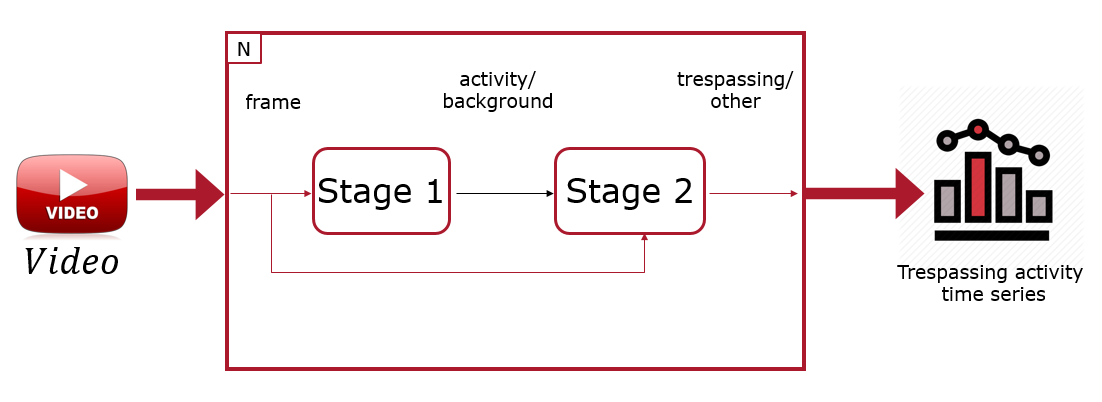
\includegraphics[width=\linewidth]{images/trespassing-detection-pipeline.PNG}
    \caption{Trespassing detection pipeline}
    \label{fig:trespassing-detection-pipeline}
\end{figure}


\subsection{Stage 1}
The goal of this stage is to filter non-activity frames from the activity frames. Thus, it is modeled as a background subtraction problem. Figure \ref{fig:background-subtraction-model} shows the block diagram of background subtraction method. 
\begin{figure}
    \centering
    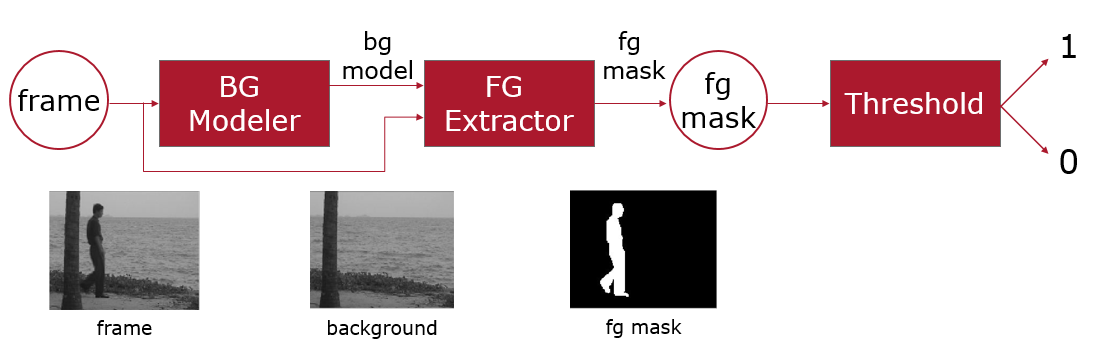
\includegraphics[width=\linewidth]{images/background-subtraction-model.PNG}
    \caption{Stage 1 - Background subtraction model}
    \label{fig:background-subtraction-model}
\end{figure}

We attempt to model the background as mixture of gaussians \cite{stauffer1999adaptive,power2002understanding}. Since, an image usually represents many different surfaces/objects, each surface/object is expected to give rise to a new gaussian. Thus all the pixel values are better represented by a mixture (sum) of gaussians. Notice that this model represents both foreground and background simultaneously. In order to apply this model to background subtraction problem, we associate each pixel with a particular surface and then associate that surface with either foreground or background. The label of each pixel (foreground/background) is determined by the label of corresponding surface. 

\subsubsection{Background (BG) modeler}
Each surface (or uniform object) that comes into the view is represented by a state $k \in {1,2,3,...,K}$. Some of these states correspond to  background while remaining ones are considered to be foreground. The process  $\mathbf{k}$ which generates the states is modeled by parameters set $\{w_1, w_2, ..., w_K\}$ where $w_k = P(k)$. Each of these parameters represents  a priori probability of surface $k$ appearing in the image. Further, $\sum_{k=1}^K w_k=1$. 

This surface process $\mathbf{k}$ is hidden and is only indirectly observable through pixel value process $X$. The pixel value process $\mathbf{X}$ is an observable random variable modeled by a gaussian process for given surface $k$. $\mathbf{X}$ is 1-D in case of gray scale images and 3-D for color images.  If $\theta_k= \{\mu_k, \Sigma_k \}$  represent the associated gaussian process then pixel value process $\mathbf{X}$ given $k$ is: 

$$ f_{\mathbf{X}|k}(X|k,\theta_k)=\frac{1}{\sqrt{(2\pi)^n |\Sigma_k |}}e^{-\frac{1}{2}(X-\mu_k)^T \Sigma_k^{-1} (X-\mu_k)} $$
where $\mu_k$ is the mean and $\Sigma_k$ is the covariance matrix of associated $k^{th}$ gaussian. 

We assume these $k$ events are disjoint so $\mathbf{X}$ can be modelled as sum of gaussians. 

$$ f_{\mathbf{X}}(X|\Phi)=\sum_{k=1}^K w_k f_{\mathbf{X}|k}(X|k,\theta_k)  $$
where $ \Phi = \{w_1, \mu_1, \Sigma_1,..., w_K, \mu_K, \Sigma_K \}$. 

\subsubsection{Foreground (FG) modeler}
In order to apply the model to background subtraction problem, first step is to determine which of the $K$ states is most likely to give rise to current pixel value $\mathbf{X}=X$. The posterior probability $P(k|X,\Phi)$ is the likelihood that pixel value $X$ was generated by surface $k$. Using the Bayes's theorem:

$$ P(k|X,\Phi) = \frac{P(k)f_{\mathbf{X}|k}(X|k,\Phi)}{f_\mathbf{X}(X,\Phi)} $$
The k which maximizes the $P(k|X,\Phi) $ is considered to be the surface associated with $X$.

$$ \hat{k}=\operatorname*{argmax}_k P(k|X,\Phi)$$

Once $X$ has been associated with a particular surface $\hat{k}$, it needs to be determined whether $\hat{k}$ is a foreground surface or background. 

The procedure for demarcation starts with ranking K states by $w_k / | \Sigma_k |$ in decreasing order. This ratio is proportional to height of weighted distribution $w_k f_{\mathbf{X}|k}(X|k,\theta_k)$. A surface $k$ is considered to be 
background if it occurs more frequently (higher $w_k$) and does not vary much (low $|\Sigma_k|$).  To separate the foreground and background surfaces, an overall prior probability $T$ of anything being in the background is used. The first $B$ of the ranked  states whose accumulated probability crosses the threshold $T$ are considered to be background. 
$$ B=\operatorname*{argmin}_b (\sum_{j=1}^b w_{j} > T)$$ 



\subsubsection{Threshold}
Output of foreground extractor is a binary mask which indicates whether a pixel belongs to foreground or not. All the foreground pixels in the image can be summed up and their ratio to the the total number of pixels in frame can be compared to a threshold value $\tau$. If the ratio is greater than threshold, then this frame is regarded as activity frame (1); otherwise it is classified as background frame (0). 


\subsection{Stage 2}
The goal of this stage is to verify human trespassing in case of activity reported by the stage 1. State-of-the-art deep learning model Faster-RCNN\cite{ref_fasterrcnn} is used to model this stage. Faster-RCNN predicts the objects (their labels and locations) corresponding to input frame. The given image is labelled with \textit{trespassing activity} if there is at least on person predicted by Faster-RCNN with corresponding confidence score greater than a threshold $\mu$. Figure \ref{fig:faster-rcnn-pipeline} shows block diagram of Faster-RCNN with detailed explanation in the following subsections. 


\begin{figure}
    \centering
    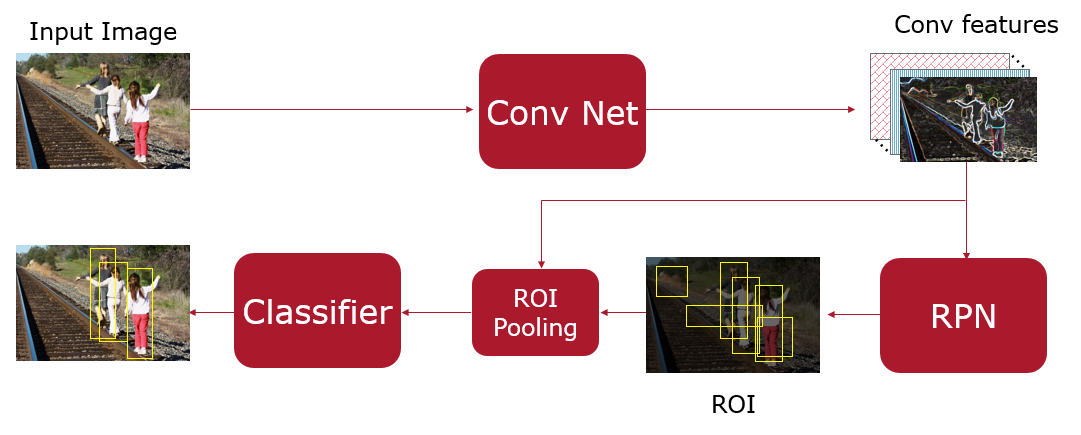
\includegraphics[width=\linewidth]{images/faster-rcnn-pipeline.PNG}
    \caption{Stage 2 - Faster-RCNN block diagram}
    \label{fig:faster-rcnn-pipeline}
\end{figure}

\subsubsection{Feature extraction (Conv. Net)}
First step is to extract convolutional features (also known as feature map) from the input frame/image. These convolutional features will be used by subsequent sub-stages as input. Due to the paramount importance of features generated by this sub-stage, it is also known as backbone of Faster-RCNN. It can be modelled as VGG\cite{simonyan2014very} or Resnet\cite{he2016deep}. We use Resnet-50 network with Feature Pyramidal Network (FPN)\cite{lin2017feature} in our experiments. 


\subsubsection{Region Proposal Network (RPN)}
This sub-stage as the name suggests is responsible for proposing regions (rectangles) potentially containing objects (people, cars etc). As seen in Figure \ref{fig:faster-rcnn-pipeline}, this sub-stage takes in the feature map and produces a list of proposals for the given image. Each proposal consists of binary label and proposed bounding box of the region of interest. The label indicates whether the proposal corresponds to an object or background. 
%The proposals thus produced by the network are subjected to non-maximum suppression. This process removes the duplicate proposals and makes subsequent processing more efficient. 

\vspace{5pt}
\textit{a. Anchors}\\
Anchor act as default region proposals. Their idea has been motivated from multi-scale sliding windows. Suppose we use a feature extraction convolutional network such that it converts a $800\times800$ image to $50\times50$ feature map (Figure \ref{fig:anchors}). This means every $(x,y)$ location on feature map corresponds to $16\times16$ patch/window on original image. Similarly, $8\times8$ window on feature map corresponds to $128\times128$ window on original image. This $8\times8$ window on feature map is known as anchor. Faster-RCNN proposes multi-scale, multi-aspect ratio anchors. A total of 3 scales (8, 16, 32 on feature map) with 3 aspect ratios ($1:1$, $1:2$, $2:1$) produces 9 anchors on each $(x,y)$ location on feature map. Since, we have $50\times50$ locations, therefore this setting produces 22,500 anchors in total. However, in practice we use less than that. All the anchors whose regions lie outside feature map (eg. anchors near edges); they don't participate in training the network. 

\begin{figure}
    \centering
    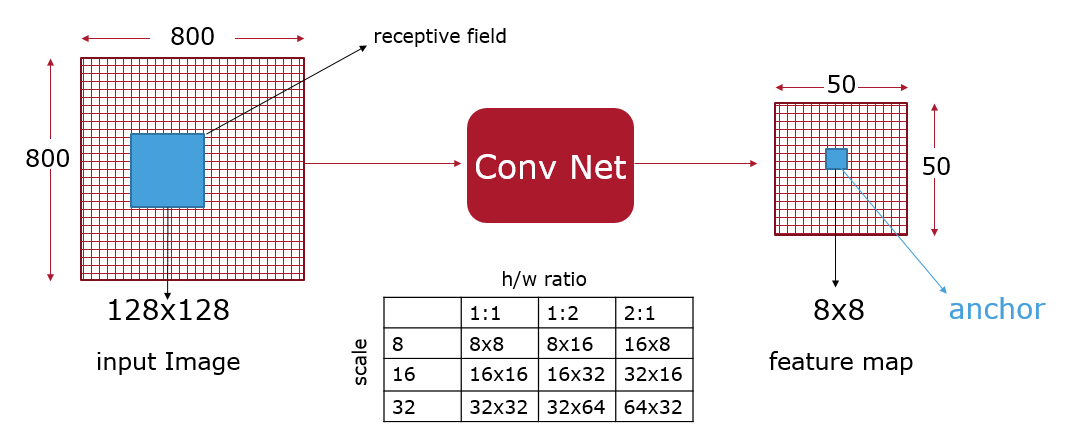
\includegraphics[width=\linewidth]{images/anchors.PNG}
    \caption[Anchor illustration]{Anchor illustration}
    \label{fig:anchors}
\end{figure}

\vspace{5pt}
\textit{b. Architecture}\\
Figure \ref{fig:RPN-architecture} shows the architecture of RPN sub-network. Input to this network is the features generated by backbone network. These features are passed through a $3\times3$ ``same\footnote{$(h,w)$ of input and output feature map remains same by automatic padding}'' convolution layer. Faster-RCNN uses 512 output feature depth for this layer. Output of this layer is fed to the bounding box regressor layer and objectness layer which predicts bounding box locations and objectness score simultaneously.
Both of these layers are modeled with $1\times1$ convolution. Bounding box regressor layer has $4k$ output depth where $k$ is the number of anchors and 4 follows from the fact that each proposal is defined by 4 scalar values. For similar reasons, objectness layer has $2k$ output features. Thus each anchor produces a proposal. All of these proposals are post-processed by Non Maximum Suppression (NMS). 


\begin{figure}
    \centering
    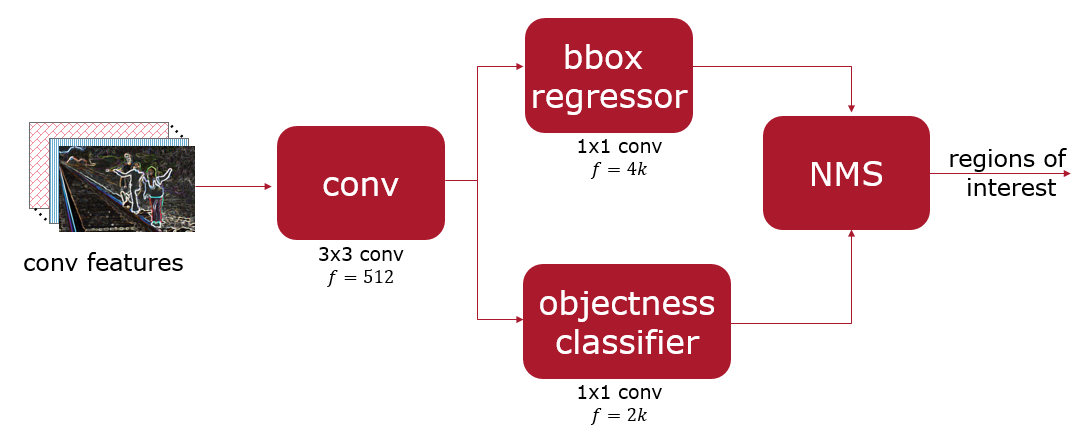
\includegraphics[width=\linewidth]{images/RPN-architecture.PNG}
    \caption[RPN architecture]{Region Proposal Network architecture}
    \label{fig:RPN-architecture}
\end{figure}



\subsubsection{Non maximum suppression (NMS)}
NMS is responsible for removing the duplicate predictions. Figure \ref{fig:nms} illustrates the goal of this process graphically. In order to suppress duplicate proposal predictions with the less confidence, first step is to sort all the proposals in descending order. The first proposal is made  the reference proposal and pushed to ``keep'' list. Intersection over Union (IoU) of this reference proposal with all the remaining proposals is computed and the proposals which sufficiently overlap with the reference proposal ($IoU > 0.7$) are discarded. They are considered to be the duplicate of reference proposal. In the next iteration, the first proposal in the list of undecided proposals is made reference proposal and the process of first iteration is repeated. Again this leads to removal of all the proposals considered to be duplicate of reference proposal. The process continues until all the proposals are decided i.e. either kept or discarded. Output of this process is the list of kept proposals. 

\begin{figure}
    \centering
    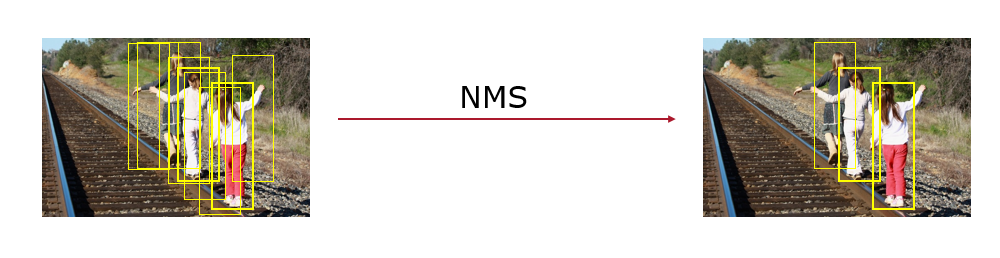
\includegraphics[width=\linewidth]{images/nms.PNG}
    \caption[Non Maximum Suppression (NMS)]{Non Maximum Suppression (NMS). Highly overlapping predictions with lesser confidence are suppressed.}
    \label{fig:nms}
\end{figure}

\subsubsection{Fast-RCNN head}
Once we have the proposals from RPN, we need to predict the corresponding objects' labels and location. Faster-RCNN uses Fast-RCNN head\cite{ref_fastrcnn} for this purpose. Fast-RCNN head has two further sub-components. First one is Region of Interest (RoI) pooling and second one is classifier layer (Figure \ref{fig:faster-rcnn-pipeline}). Input to the Fast-RCNN head will be feature map and list of kept proposals, and output shall be improved bounding box locations of corresponding proposals along with class labels. 

Different proposals have different feature map sizes. However, the classifier expects them to be of same size. This process (RoI pooling) is responsible for converting variable sized feature maps into fixed sized. The methodology used by Fast-RCNN in this case is quite simple. Suppose a feature map of size $8\times 8$ has to be converted to $2 \times 2$ size. Then, a grid of size $2 \times 2$ is placed on top of feature map such that its boundaries align with the feature map. The maximum feature value from each grid cell is copied to corresponding cell in output buffer. This converts a $8\times 8$ feature map to a size of $2 \times 2$.

Once RoI pooling has adjusted the size of feature map to fixed dimensions, the feature maps are ready to be fed to classifier. The classifier takes in those features and pass them through two fully connected layers. The output of those two layers is fed to two separate fully connected layers responsible for predicting bounding boxes and object class labels. The bounding boxes and labels so predicted are the final output of Faster-RCNN. Figure \ref{fig:classifier} illustrates the architecture of classifier.

\begin{figure}
    \centering
    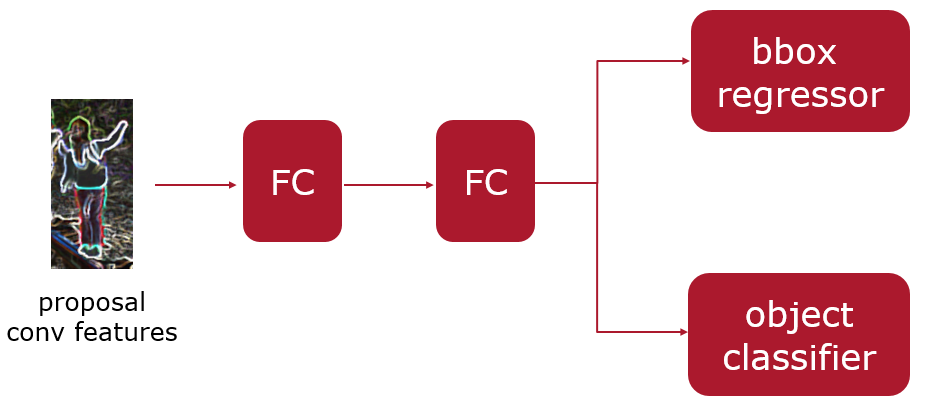
\includegraphics[width=\linewidth]{images/classifier.PNG}
    \caption{Fast-RCNN classifier}
    \label{fig:classifier}
\end{figure}

\subsubsection{Training loss}
While training the Faster-RCNN, we train two sub-networks: RPN and classifier. Both of these networks have two objectives: label classification and bounding box regression. Following two equations indicate the RPN and classifier loss. First term corresponds to label classification and second term corresponds to bounding box regression. 

$$Loss_{RPN}= \frac{1}{N_{cls}}\sum_i L_{cls}(\hat{p}_i,p_i) + \frac{\lambda_r}{N_{reg}}\sum_i p_i L_{reg}(\hat{t}_i,t_i)$$

\begin{small}
$$Loss_{cla} = \frac{1}{N_{cls}}\sum_i L_{cls}(\hat{q}_i,q_i) + \frac{\lambda_c}{N_{reg}}\sum_i [q_i > 0] L_{reg}(\hat{u}_i,u_i)$$
\end{small}
where \\
$\hat{p}_i=$ anchor label prediction \\
$\hat{t}_i=$ anchor bounding box prediction \\
$\hat{q}_i=$ RoI label prediction \\
$\hat{u}_i=$ RoI bounding box prediction \\
${p}_i=$ anchor ground truth label \\
${t}_i=$ anchor ground truth bounding box  \\
${q}_i=$ RoI ground truth label  \\
${u}_i=$ RoI ground truth bounding box  \\
$\lambda_r =$ RPN loss balance coef. \\
$\lambda_c =$ classifier loss balance coef. \\
$N_{cls}=$ mini-batch size \\
$N_{reg}=$ total anchors

Classification loss $L_{cls}$ is the standard log loss and regression loss $L_{reg}$ is the smooth-$L_1$ loss as defined below. 

$$ L_{cls}(\hat{y},y) = -\sum_j y_jlog(\hat{y}_j) $$
$$ L_{reg}(\hat{b},b) = \sum_{j=1}^4 SL_1(\hat{b}_j - b_j) $$
$$SL_1(x) = \begin{cases}
0.5x^2, & \text{if } |x|<1 \\
x-0.5,  & \text{otherwise}
\end{cases}
$$
where input parameters to each function carry standard meaning. 

Total loss of the network is simply the sum of RPN loss and classifier loss.
$$ Loss = Loss_{RPN} + Loss_{cla} $$

Apart from that notice the term $p_i$ in regression term of RPN loss. This makes sure that regression loss is activated only if proposal corresponds to an object, not the background.  Thus bounding box predictions corresponding to background proposals do not contribute towards training. Furthermore, the expression $[q_i>0]$ does a similar job in classifier loss. This again acts as a flag to add regression loss only corresponding to actual objects and not the background. 

$\lambda_r$ and $\lambda_c$ act as the balancing parameter  between label classification and bounding box regression. The authors of Faster-RCNN claim that $\lambda_r$ is redundant and Faster-RCNN remains insensitive to a large range of $\lambda_r$. 


\section{Experimental evaluation}
\label{sec:exp-eval}
\subsection{Dataset}
The dataset we used for experimental evaluation is VIRAT 2.0 \cite{virat20}. This dataset targets activity classification and is thus enriched with human activity, meaning all the frames mostly contain humans in motion. On the other hand, trespassing data is known to be extremely sparse. Therefore, we augment the VIRAT 2.0 dataset to control the amount of activity to background ratio as described below: 

\vspace{5pt}
\subsubsection{Synthetic dataset generator}
Figure \ref{fig:synthetic-dataset-generator} illustrates the black box model of our synthetic dataset generator. We adopt the following steps to generate the synthetic data: 
\begin{enumerate} 
    \item identify background frame
    \item make background block(s)
    \item write background block(s)
    \item write activity block(s)
    \item repeat (3) and (4)
\end{enumerate}

\begin{figure}
    \centering
    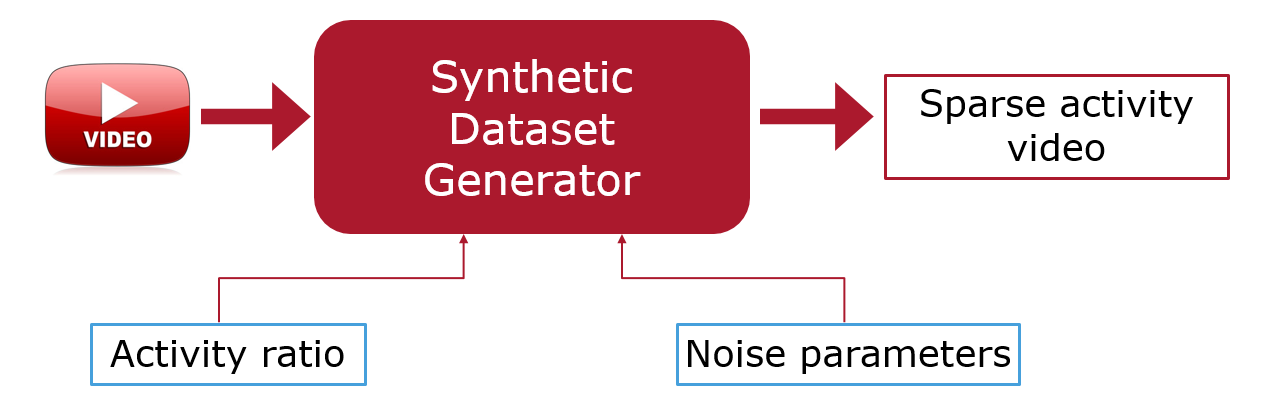
\includegraphics[width=\linewidth]{images/synthetic-dataset-generator.PNG}
    \caption{Synthetic dataset generator}
    \label{fig:synthetic-dataset-generator}
\end{figure}

Step 1 is human labor intensive but simple. We manually scroll through a video and identify a variety of frames with no human. We call these frames, the background frames. In step 2, we repeat each background frame $\Delta \times fps$ times to generate corresponding background block. Here, the $fps$ denotes the frames-per-second of the original video and $\Delta$ indicates the target length of background block in seconds. In step 3, we randomly select a certain number of  background blocks (determined in step 2) and write them to output video stream. Exact number of background blocks written depend on activity ratio, discussed at the end of this subsection. Step 4 writes the activity block in output video stream. An activity block is simply a section of the original video. By default, we use $30s$ long activity blocks. Length of each background block is also kept at $30s$ by default. Figure \ref{fig:synthetic-video} helps understand the concept of activity block and synthetic video.  

\begin{figure}
    \centering
    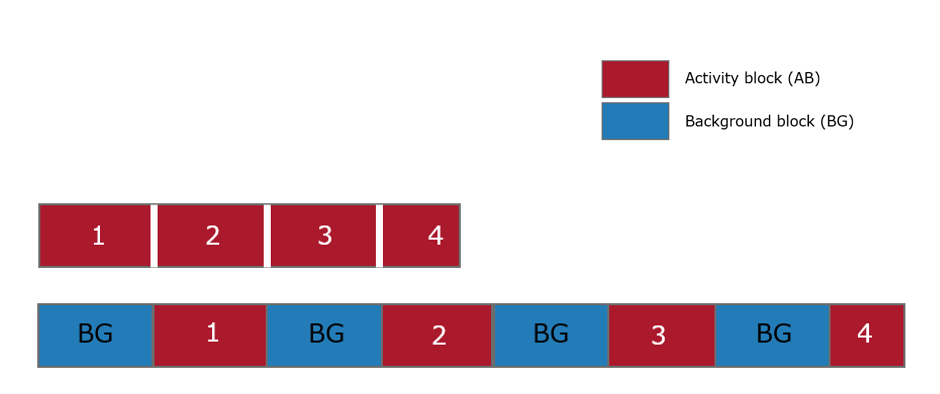
\includegraphics[width=\linewidth]{images/synthetic-video.PNG}
    \caption{Synthetic video illustration}
    \label{fig:synthetic-video}
\end{figure}

An important metric associated with this procedure is \textit{Activity Ratio}. It captures the fraction of activity present in the output synthetic video. It is defined as: 
$$ \text{Activity Ratio} = \text{AR} = \frac{1}{1+nBG} $$
where $nBG=$ number of background blocks per activity block. Figure \ref{fig:synthetic-video} has $nBG=1$. Table \ref{table:activity-ratio} explains the relationship between $nBG$ and AR. 


\begin{table}
\centering
\caption{Relationship of number of background blocks and activity ratio} \vspace{5pt}
\label{table:activity-ratio}
\begin{tabular}{@{}| l | l | l | @{}} \hline
nBG & nAB:nBG & AR   \\ \hline \hline
1   & 1:1     & 0.5  \\
3   & 1:3     & 0.25 \\
5   & 1:5     & 0.16 \\ \hline
\end{tabular}
\end{table}

\subsubsection{Adding noise}
Outdoor surveillance videos are often subjected to environmental challenges such as rain and snow. In order to test the robustness of our approach in those challenging situations, we add noise to our synthetic data. Salt and pepper noise \cite{marques2011practical} is known for modelling the rain and snow effect, therefore we use it in our experiments. 
Table \ref{table:noise-params} describes the parameters that control the level of noise. 

In order to add noise, we first select $p\%$ of frames from each background block. Each of the frames is equally likely to be selected. Now we draw an integer $r$ from the normal distribution with parameters $\mu$ and $\sigma$. For each selected frame, we select $r$ pixels and add noise to them. Again all pixels are equally likely. 

\begin{table}
\centering
\caption{Noise parameters}  \vspace{5pt}
\label{table:noise-params}
\begin{tabular}{|l|l|}
\hline
params & description                              \\ \hline \hline
$p$          & percentage of noisy frames in BG block  \\ 
$\mu$        & avg. number of noisy pixels in noisy frame     \\ 
$\sigma$     & standard deviation of number of noisy pixels     \\ \hline
\end{tabular}
\end{table}

\subsection{Experiments and discussion}
In order to validate our approach, we carry out an extensive and in depth experimental evaluation.  We study our proposed approach from three different perspectives: 

\begin{enumerate}
\item time-accuracy trade-off
\item stage-wise analysis
\item noise analysis
\end{enumerate}

We shall start by discussing time-accuracy trade-off. This allows us to study end-to-end performance of pipeline while trading off computational time.  We also do stage-wise analysis where each stage is evaluated independently of other. This helps us understand which stage is acting as bottleneck in terms of performance. Additionally, we also do noise analysis to understand the robustness of system to noise.

\subsubsection{Time-accuracy trade-off experiment}
In time-accuracy trade off experiment, we study how the data can be processed in less time by compromising performance. We vary certain control parameters (stage 1 threshold in this case) and observe the time it takes to process the data along with the performance of the complete pipeline. Figure \ref{fig:time-acc-tradeoff-ar-mog} shows time-accuracy trade off for varying activity ratios (AR). The trade off curve depicts f1 score on y-axis and normalized processing time on the x-axis. Normalized processing time is defined as: 
$$\text{normalized time} = \frac{\text{total time to process video data}}{\text{length of video data}}$$
It is clear (in Figure \ref{fig:time-acc-tradeoff-ar-mog}) that as the f1 score goes up, the normalized processing time also goes up, indicating the trade off. Notice that as the AR decreases, the trade off curve shifts to the left. This is because in less active environment (low AR), stage 1 is able to filter out more frames and thus less frames need to be processed by stage 2. Thus the curve shifts to the left indicating less overall processing time.   

For any curve (in Figure \ref{fig:time-acc-tradeoff-ar-mog}) with a given AR, top right point corresponds to small value of stage 1 threshold ($\tau$). As $\tau$ is increased, we move towards the left; consuming less time at the cost of performance . This is expected as stage 1 filters more and more frames with increasing threshold ($\tau$) and thus lesser frames are processed by stage 2.The synthetic dataset parameters used in this experiment are shown in table \ref{table:fig1_data_params}. 

\begin{figure}
    \centering
    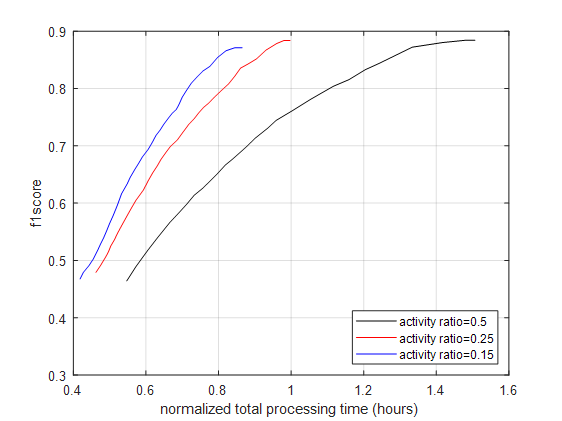
\includegraphics[width=\linewidth]{images/time-acc-tradeoff-ar-mog.png}
    \caption{Time-accuracy trade off for varying AR}
    \label{fig:time-acc-tradeoff-ar-mog}
\end{figure}

\begin{table}
\centering
\caption{Synthetic data parameters for time-accuracy trade off} \vspace{5pt}
\label{table:fig1_data_params}
\begin{tabular}{|l|l|}
\hline
parameter             & value  \\ \hline \hline
p                     & 1\%    \\ 
$\mu$    & 0.50\% \\ 
$\sigma$ & 0.20\% \\ \hline
\end{tabular}
\end{table}

\subsubsection{Stage-wise analysis experiments}
In this part, we analyse both stage 1 and 2 independently. F1 score is primarily used for analysis as it helps in selecting optimum operating threshold. Apart from that, we use AUC (Area Under the Curve) as the evaluation metric since it is not affected by class imbalance. We naturally have class imbalance since very few trespassing frames exist as compared to other frames. Table \ref{table:auc-time-analysis-s1} shows AUC and mean processing time for both stages. Stage 1 has AUC of 0.94 whereas stage 2 shows an AUC of 0.81. The first stage takes 30 ms  (on average) to process a frame while stage 2 takes around 500 ms on $1080 \times 960$ sized frame. This shows that stage 1 is approx. $16.7$ times faster than stage 2 which resonates with our goal stated in section \ref{sec:goal}. 

Figure \ref{fig:f1-analysis-mog} shows how f1 score of stage 1 changes w-r-t threshold $\tau$ (percentage of foreground pixels). At $0.1\%$, it achieves maximum f1 score of 0.91. Therefore, the stage 1 should be operated at this threshold.

\begin{figure}
    \centering
    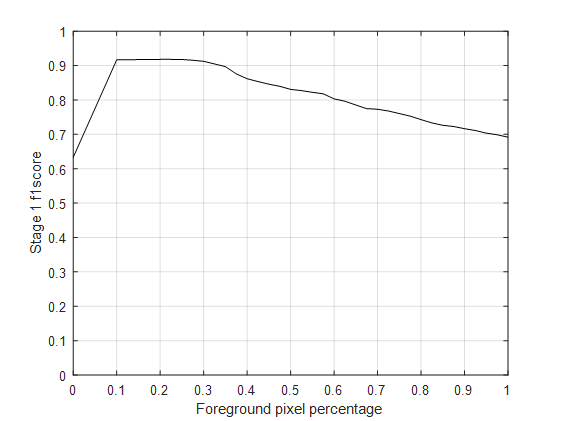
\includegraphics[width=\linewidth]{images/f1-analysis-mog.png}
    \caption{Stage 1 evaluation}
    \label{fig:f1-analysis-mog}
\end{figure}

Figure \ref{fig:f1-analysis-s2} shows the f1 score variation for stage 2. Y-axis indicates f1 score whereas x-axis varies prediction probability threshold $\nu$. It is clear that maximum f1 score of 0.89 is achieved on $\nu=0.3$. Therefore, stage 2 should be operated at this threshold.

Note that Faster-RCNN, which is the backbone of our stage 2, produces multiple object predictions corresponding to each input image\footnote{image and frame have been used interchangeably in this text}. However, we model our problem as a binary classification of input frame as trespassing activity frame or other frame. Therefore, we need to map Faster-RCNN predictions to binary labels i.e. trespassing or other. We achieve this mapping by the following definition:

$$
\text{prediction} = 
\begin{cases}
% 1, &    \text{\footnotesize{if there is at least one valid person detection}} \\
1, &    \text{if any valid person detection exists} \\
0, &    \text{otherwise}
\end{cases}
$$
where \\
$\text{valid person detection} = \hat{p}_i>\nu \quad \& \quad IoU(\hat{b}_i,b_j)>0.5$ \\
$\hat{b}_i =i^{th} \text{ prediction bounding box}$ \\
$b_j =j^{th} \text{ ground truth bounding box}$ \\
$\hat{p}_i = i^{th} \text{prediction probability}$ \\
$\nu =  \text{prediction probability threshold}$

\begin{figure}
    \centering
    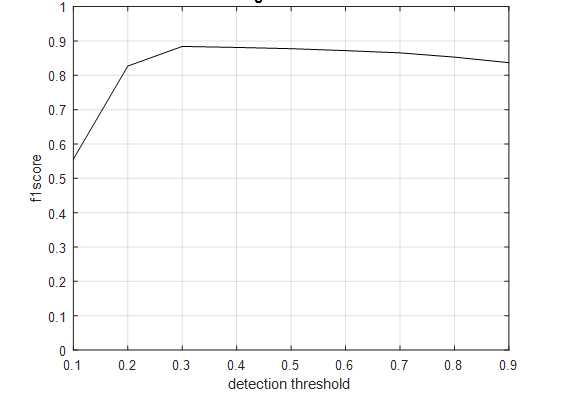
\includegraphics[width=\linewidth]{images/f1-analysis-s2.png}
    \caption{Stage 2 evaluation}
    \label{fig:f1-analysis-s2}
\end{figure}



\begin{table}
\centering
\caption{Stage 1 AUC and time analysis} \vspace{5pt}
\label{table:auc-time-analysis-s1}
\begin{tabular}{|l|l|c|}
\hline
stage   	& AUC     & mean processing \\
            &         &  time (ms)  \\ \hline \hline
stage 1     & 0.94    & 30    \\
stage 2     & 0.81    & 500  \\ \hline
\end{tabular}
\end{table}


\subsubsection{Noise analysis experiments}
Third and final part of our experimental evaluation is noise analysis. In this part, we evaluate the robustness of stage 1 against noise. In terms of noise, we have 3 parameters: $p, \mu, \text{ and } \sigma$. Description of these parameters has been discussed in table \ref{table:noise-params}. To study the influence of one parameter, we vary it while keeping the others constant. 

Table \ref{table:noise-analysis-auc-mog} shows AUC for stage 1 varying $p$ and $\mu$. We use the noise parameters ($AR=0.5$, $\mu=0.5\%$, $\sigma=0.2\%$) while varying $p$ and ($AR=0.5$, $p=2\%$, $\sigma=0.2\%$) while varying $\mu$. For both $p$ and $\mu$, it is clear that increase in noise level decreases the AUC of stage 1.  This result is also verified by f1 score plot of stage 1. Figure \ref{fig:noise-analysis-mog-p} and \ref{fig:noise-analysis-mog-mu} show the effect of change in $p$ and $\mu$ respectively. Figure \ref{fig:noise-analysis-mog-p} shows that as $p$ increases, the whole f1 score curve shifts downward. This indicates the degradation of performance with increase in $p$. Similar observation can also be made in figure \ref{fig:noise-analysis-mog-mu} (showing the effect of change in $\mu$); however, the change is less prominent in this case.  


\begin{table}
\centering
\caption{Noise analysis - AUC for varying $p$ and $\mu$} \vspace{5pt}
\label{table:noise-analysis-auc-mog}

\begin{tabular}{l r}

\begin{tabular}{|l|l|}
\hline
$p$         & AUC  \\ \hline \hline
2\%         & 0.93   \\
4\%         & 0.87    \\ 
6\%         & 0.83      \\ 
8\%         & 0.78       \\ \hline
\end{tabular}


\begin{tabular}{|l|l|}
\hline
$\mu$         & AUC  \\ \hline \hline
0.5\%         & 0.93   \\
0.7\%         & 0.92    \\ 
0.9\%         & 0.91      \\ 
1.1\%         & 0.88       \\ \hline
\end{tabular}

\end{tabular}

\end{table}

\begin{figure}[ht]
    \centering
    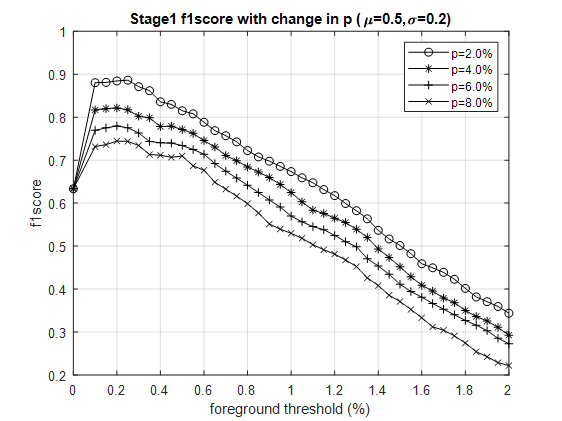
\includegraphics[width=\linewidth]{images/noise-analysis-mog-p.png}
    \caption{Noise analysis - varying $p$}
    \label{fig:noise-analysis-mog-p}
\end{figure}

\begin{figure}[ht]
    \centering
    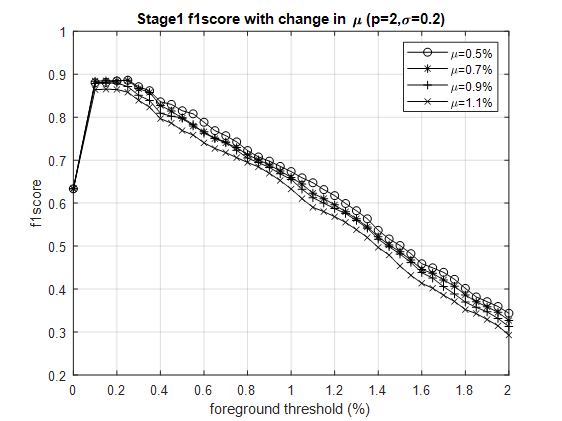
\includegraphics[width=\linewidth]{images/noise-analysis-mog-mu.png}
    \caption{Noise analysis - varying $\mu$}
    \label{fig:noise-analysis-mog-mu}
\end{figure}
\section{Conclusion and future work}
\label{sec:conclusion}
In this work, we propose and then comprehensively study a flexible trespassing detection solution framework (called ARTS) adopting state-of-the-art deep learning methods. The proposed framework can trade-off processing speed and accuracy. Although initially envisioned for railroad security, the proposed approach has potential applications in video surveillance domains characterized by a sparsity in activity.  The ARTS framework features two stages with the first stage designed to efficiently remove the background frames from the activity frames. The second stage is responsible for differentiating between human trespassing and any other unknown activity. Our proposed ARTS framework adapts a plug and play infrastructure to allow researchers to plug in other algorithms relevant to stage 1 or to stage 2, with ease in the future. The effectiveness of our approach has been demonstrated on a public domain surveillance dataset. 

Future directions include building a trespassing prediction system that uses the output of the ARTS to predict future trespassing events. Another direction is to improve the accuracy of the proposed techniques. We note that the current accuracy is limited by the accuracy of stage 2. Currently stage 2 does not use any temporal information, i.e., each frame is treated independently and thus not conditioned on the previous frames (history). The utilization of the temporal information has the potential of significantly improving the accuracy specially for challenging cases of occlusion and background.

\bibliographystyle{plain}
\bibliography{references}

\end{document}
